\chapter{Specifikacija programske potpore}
		
	\section{Funkcionalni zahtjevi}
			
		
			
			
			\noindent \textbf{Dionici:}
			
			\begin{packed_enum}
				
				\item Korisnici aplikacije
				\item Klijenti aplikacije				
				\item Zaposlenici aplikacije
					\begin{packed_enum}
					
					\item Trener
					\item Članovi uprave
					\end{packed_enum}
				\item Administrator
				\item Razvojni tim
				
				
			\end{packed_enum}
			
			\noindent \textbf{Aktori i njihovi funkcionalni zahtjevi:}
			
			
			\begin{packed_enum}
				\item  \underbar{Neregistrirani/Neprijavljeni korisnik(inicijator) može:}
				
				\begin{packed_enum}
					
					\item pregledavati sadržaj web aplikacije
					\item dodavati artikle u košaricu web shop-a, brisati jedan ili sve, pregledavati košaricu
					\item registrirati se, tj. napraviti novi korisnički račun s potrebnim podacima
					\item promijeniti jezik aplikacije				
				\end{packed_enum}
			
				\item  \underbar{Klijent aplikacije može:}
				
				\begin{packed_enum}
					
					\item sve što može neregistrirani korisnik osim registracije
					\item pregledavati i mijenjati osobne podatke
					\item izbrisati svoj korisnički račun
					\item platiti narudžbu
					\item ostaviti recenziju na web shop-u
					\item koristiti prijenos utakmica uživo
					\item koristiti chat uslugu pri gledanju prijenosa uživo
					
				\end{packed_enum}
			\item  \underbar{Trener, odnosno upravitelj kluba (inicijator) može:}
			
			\begin{packed_enum}
				
				\item dodavati sadržaj na stranicu, brisati ili mijenjati postojeći
				\item dodati novog igrača
				\item promijeniti podatke postojećem igraču
				\item izbrisati igrača iz kluba
				
			\end{packed_enum}
		\item  \underbar{Član uprave (inicijator) može:}
		
		\begin{packed_enum}
			
			\item pregledati aktivne narudžbe
			\item označiti narudžbu zaprimljenom
			\item uređivati artikle na web shop-u
			\item dodati artikl u web shop
			\item dodati popuste na web shop
			
		\end{packed_enum}
	
	\item  \underbar{Aministrator aplikacije (inicijator) može:}
	
	\begin{packed_enum}
		
		\item dodavati nove račune (trenera, administratora i upravu)
		\item brisati račune
		\item brisati recenzije
		\item pregledavati klijente
		\item promijeniti prava pristupa
	
	\end{packed_enum}
\item  \underbar{Baza podataka (sudionik):}

\begin{packed_enum}
	
	\item pohranjuje sve podatke o korisnicima i njihovim ovlastima
	\item pohranjuje sve podatke o sadržaju, ponudi i količinama

	
\end{packed_enum}
		\item  \underbar{Banka (sudionik):}
		
		\begin{packed_enum}
			
			\item provjerava, odnosno vrši transakcije prilikom plaćanja u web shop-u
			
			
		\end{packed_enum}
			\end{packed_enum}
			
			\eject 
			
			
				
			\subsection{Obrasci uporabe}
				
				
					

					\noindent \underbar{\textbf{UC1: Pregled web stranice}}
					\begin{packed_item}
	
						\item \textbf{Glavni sudionik: } Korisnik, klijent
						\item  \textbf{Cilj:} Pregledati sadržaj web stranice, uključujući web shop
						\item  \textbf{Sudionici:} Baza podataka
						\item  \textbf{Preduvjet:} -
						\item  \textbf{Opis osnovnog tijeka:}
						
						\item[] \begin{packed_enum}
	
							\item 1. Stranica je prikazana tijekom pokretanja aplikacije
							\item Korisnik ili klijent pregledava sadržaj (Kontak, O nama, ...)
						\end{packed_enum}
						
						\item  \textbf{Opis mogućih odstupanja:}
						
						\item[] \begin{packed_item}
	
							\item[2.a] $<$opis mogućeg scenarija odstupanja u koraku 2$>$
							\item[] \begin{packed_enum}
								
								\item $<$opis rješenja mogućeg scenarija korak 1$>$
								\item $<$opis rješenja mogućeg scenarija korak 2$>$
								
							\end{packed_enum}
							\item[2.b] $<$opis mogućeg scenarija odstupanja u koraku 2$>$
							\item[3.a] $<$opis mogućeg scenarija odstupanja  u koraku 3$>$
							
						\end{packed_item}
						\end{packed_item}
					
					
					
				
				
					
				\subsubsection{Dijagrami obrazaca uporabe}
					
					\textit{Prikazati odnos aktora i obrazaca uporabe odgovarajućim UML dijagramom. Nije nužno nacrtati sve na jednom dijagramu. Modelirati po razinama apstrakcije i skupovima srodnih funkcionalnosti.}
					
					\begin{figure}[H]
						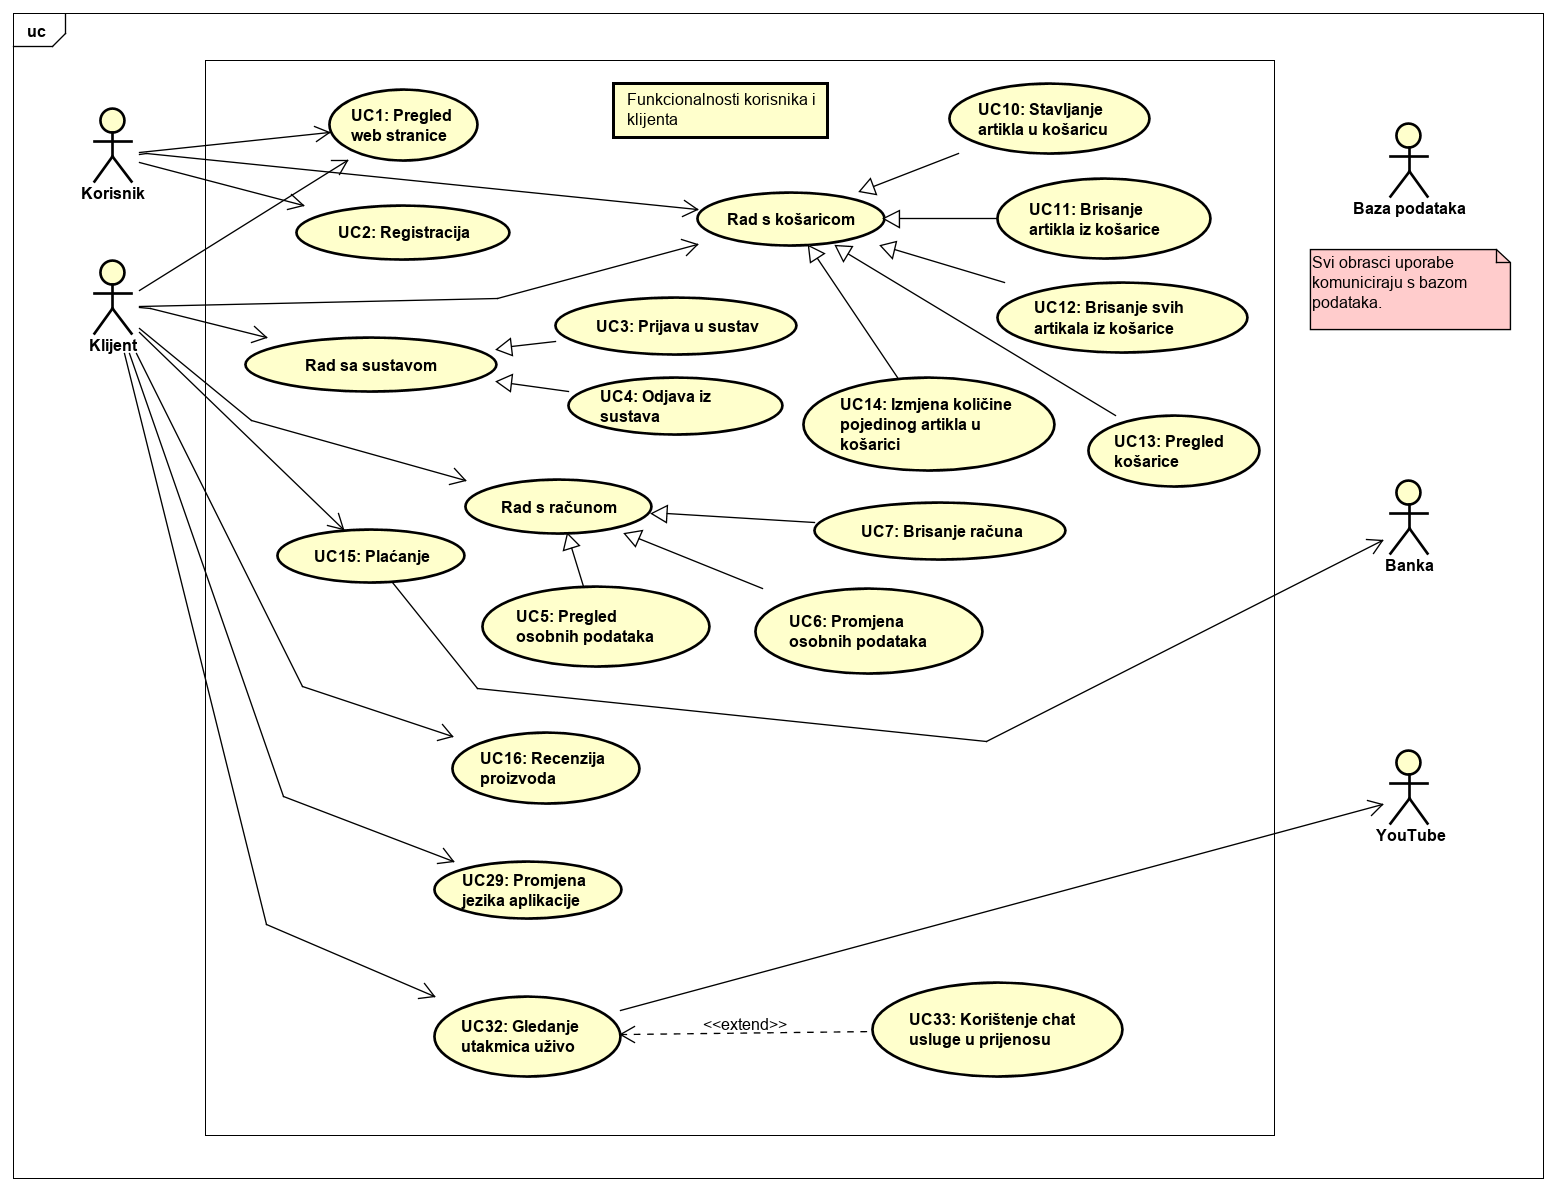
\includegraphics[width=\linewidth]{dijagrami/Funkcionalnosti_korisnika_i_klijenta.png}
						\centering
						\caption{Funkcionalnosti korisnika i klijenta}
						\label{fig:UseCaseDiagram1}
					\end{figure}
				
					\begin{figure}[H]
						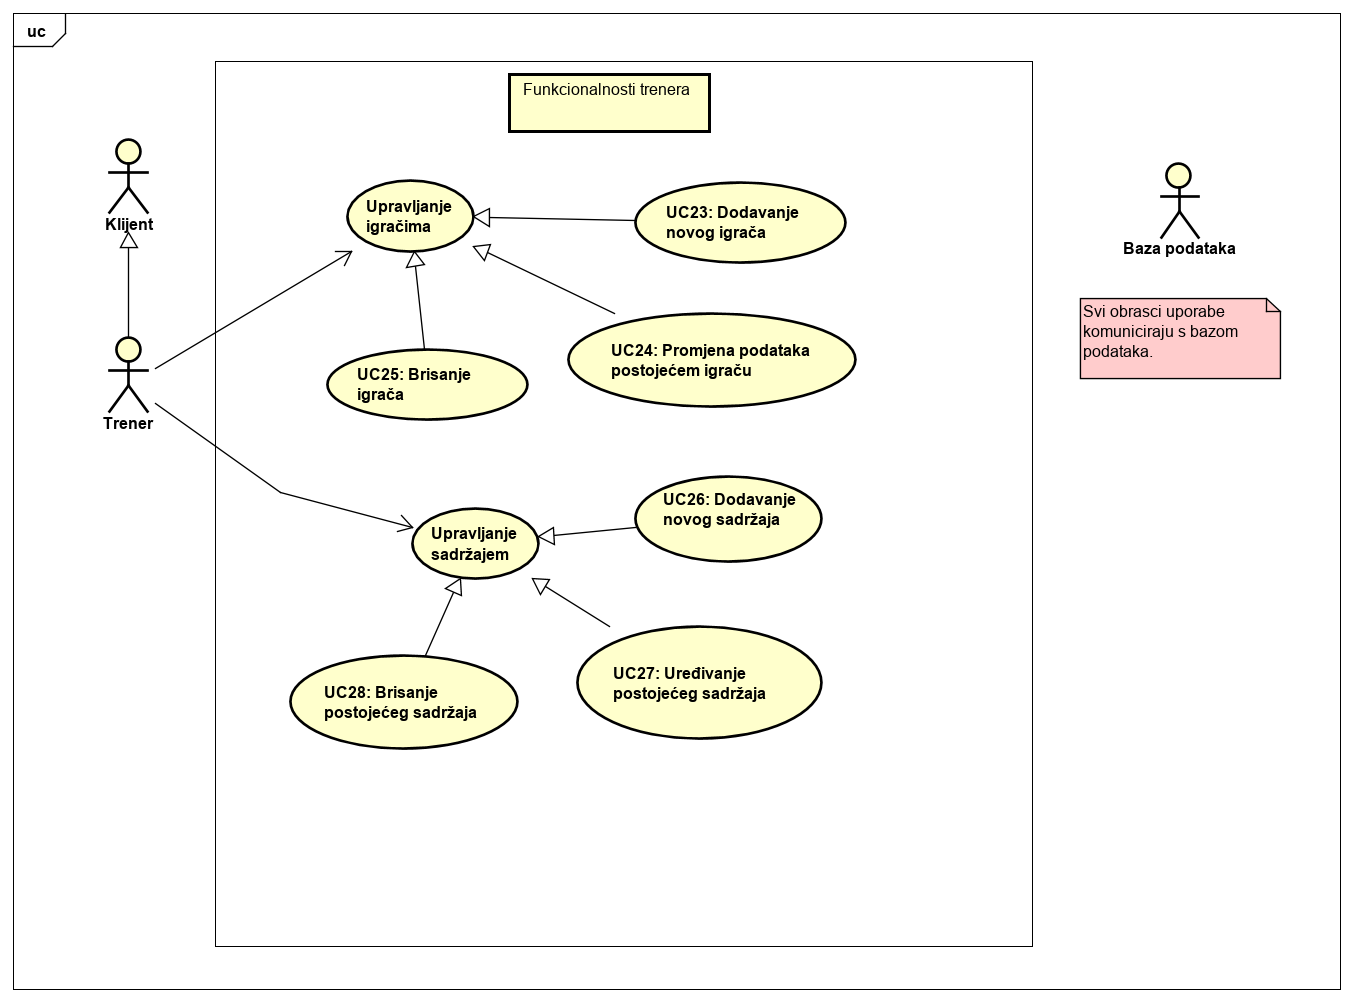
\includegraphics[width=\linewidth]{dijagrami/Funkcionalnosti_trenera.png}
						\centering
						\caption{Funkcionalnosti trenera}
						\label{fig:UseCaseDiagram2}
					\end{figure}
				
					\begin{figure}[H]
						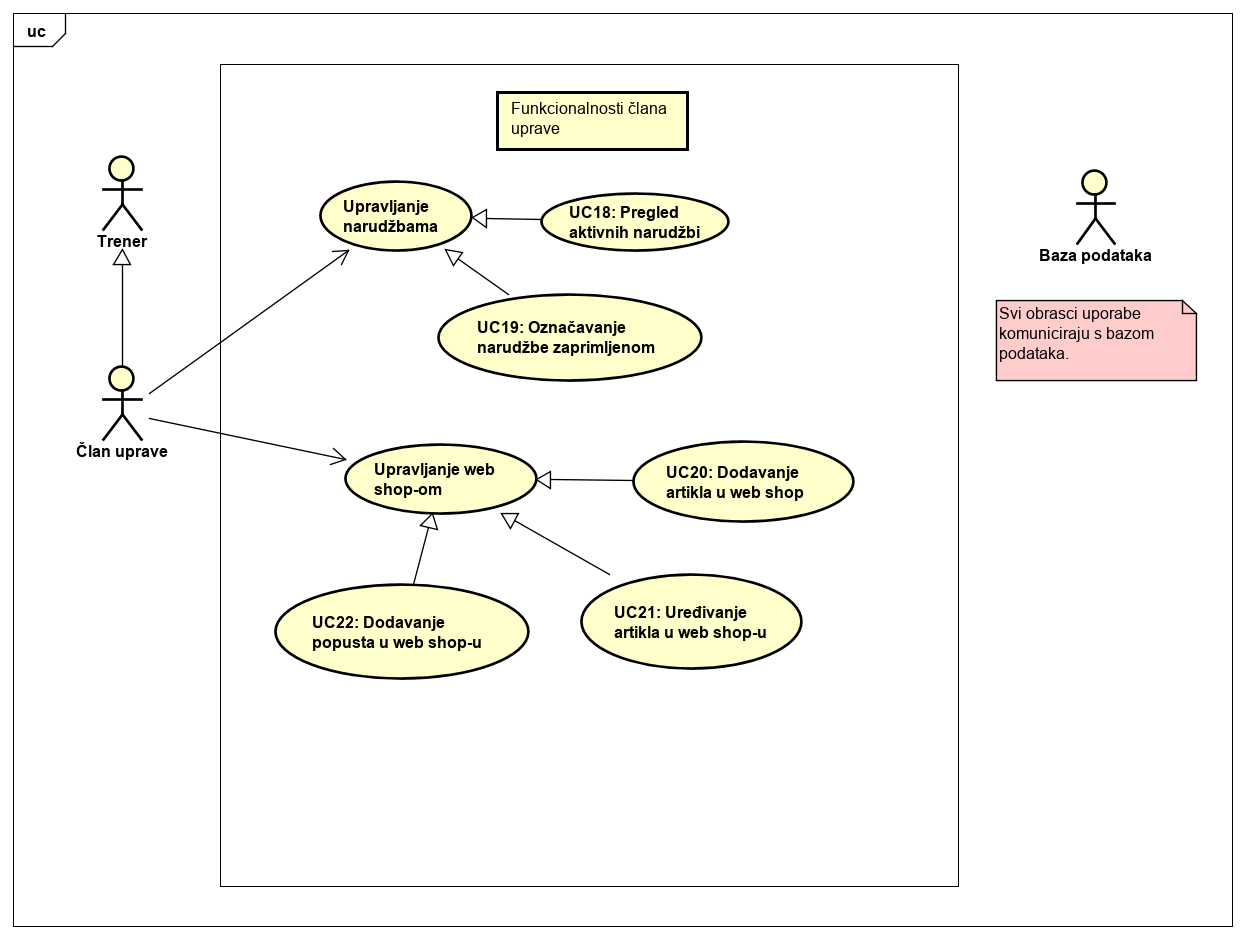
\includegraphics[width=\linewidth]{dijagrami/Funkcionalnosti_clana_uprave.png}
						\centering
						\caption{Funkcionalnosti člana uprave}
						\label{fig:UseCaseDiagram3}
					\end{figure}
				
					\begin{figure}[H]
						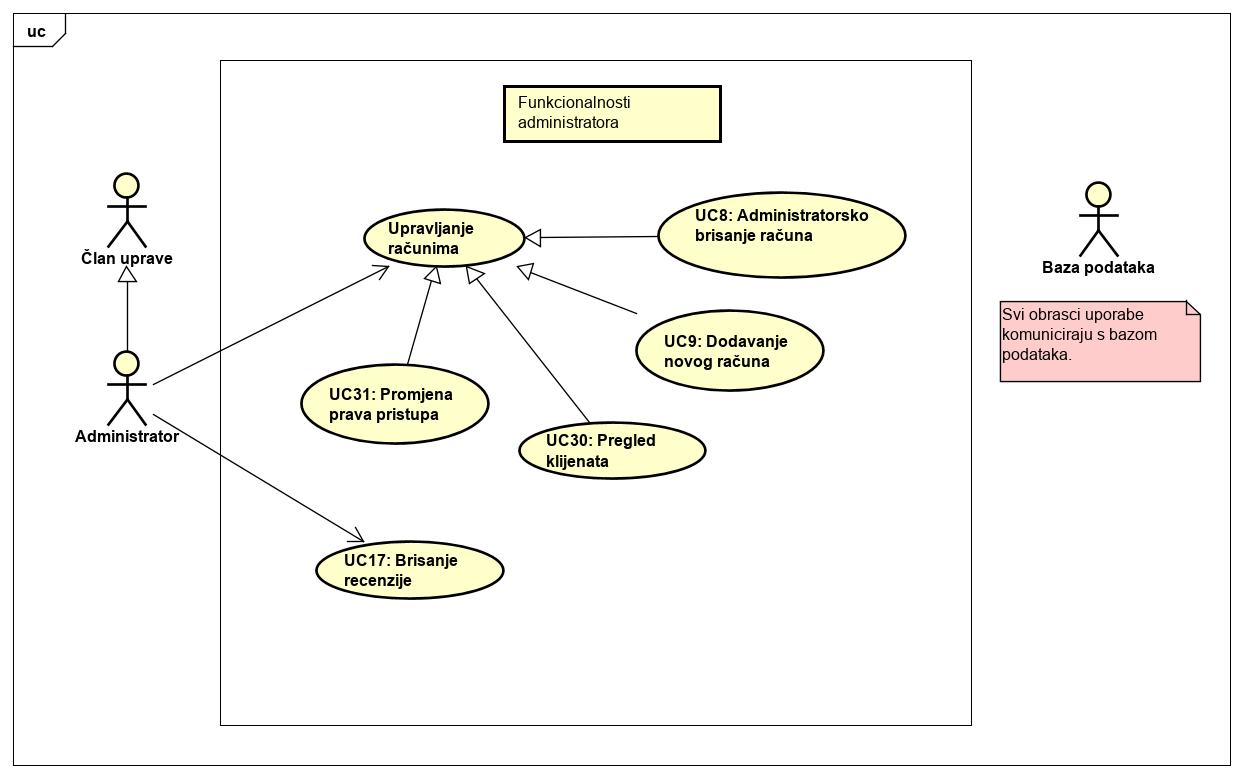
\includegraphics[width=\linewidth]{dijagrami/Funkcionalnosti_administratora.png}
						\centering
						\caption{Funkcionalnosti administratora}
						\label{fig:UseCaseDiagram4}
					\end{figure}
				
				\eject		
				
			\subsection{Sekvencijski dijagrami}
				
				\textbf{\textit{dio 1. revizije}}\\
				
				\textit{Nacrtati sekvencijske dijagrame koji modeliraju najvažnije dijelove sustava (max. 4 dijagrama). Ukoliko postoji nedoumica oko odabira, razjasniti s asistentom. Uz svaki dijagram napisati detaljni opis dijagrama.}
				\eject
				
				\begin{figure}[H]
					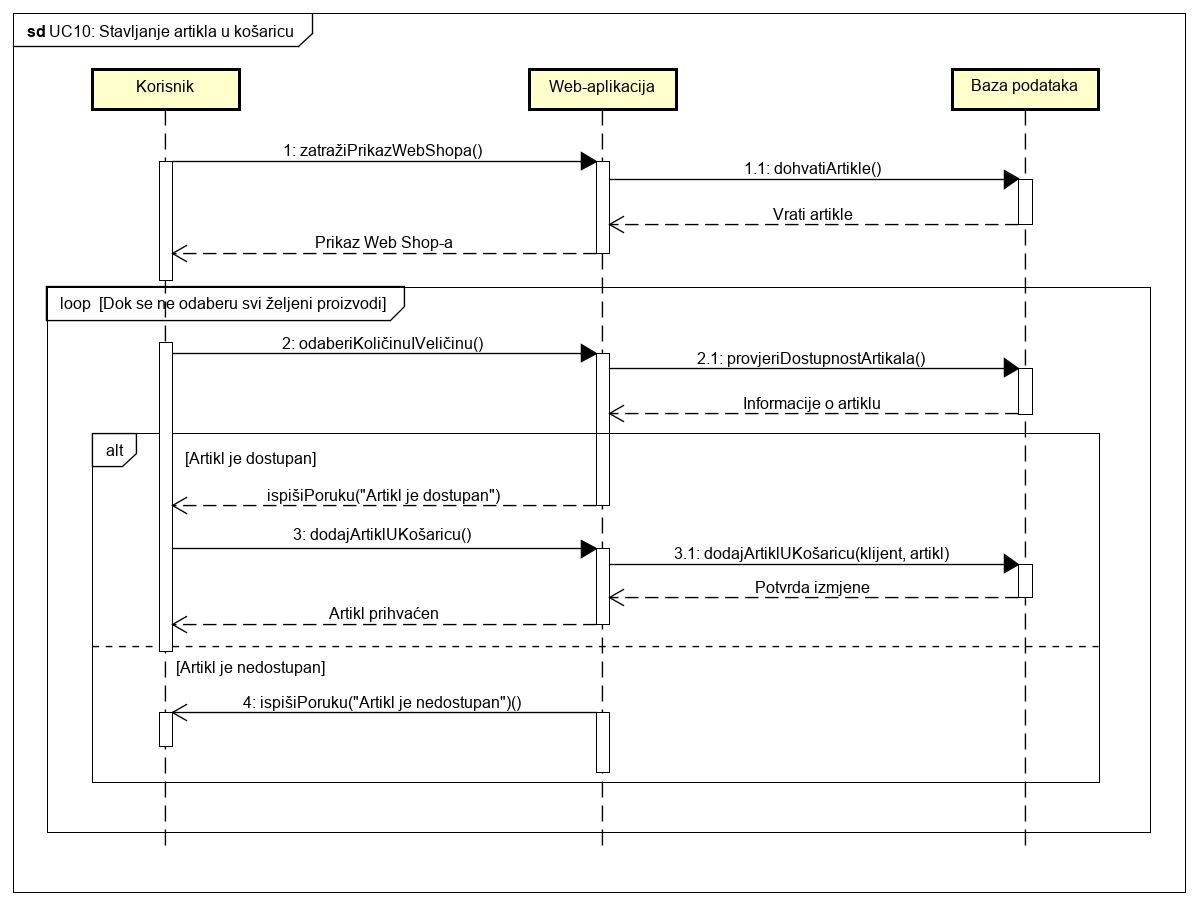
\includegraphics[width=\linewidth]{dijagrami/UC10.png}
					\centering
					\caption{UC10, Stavljanje artikla u košaricu}
					\label{fig:SequanceDiagram1}
				\end{figure}
			
				\begin{figure}[H]
					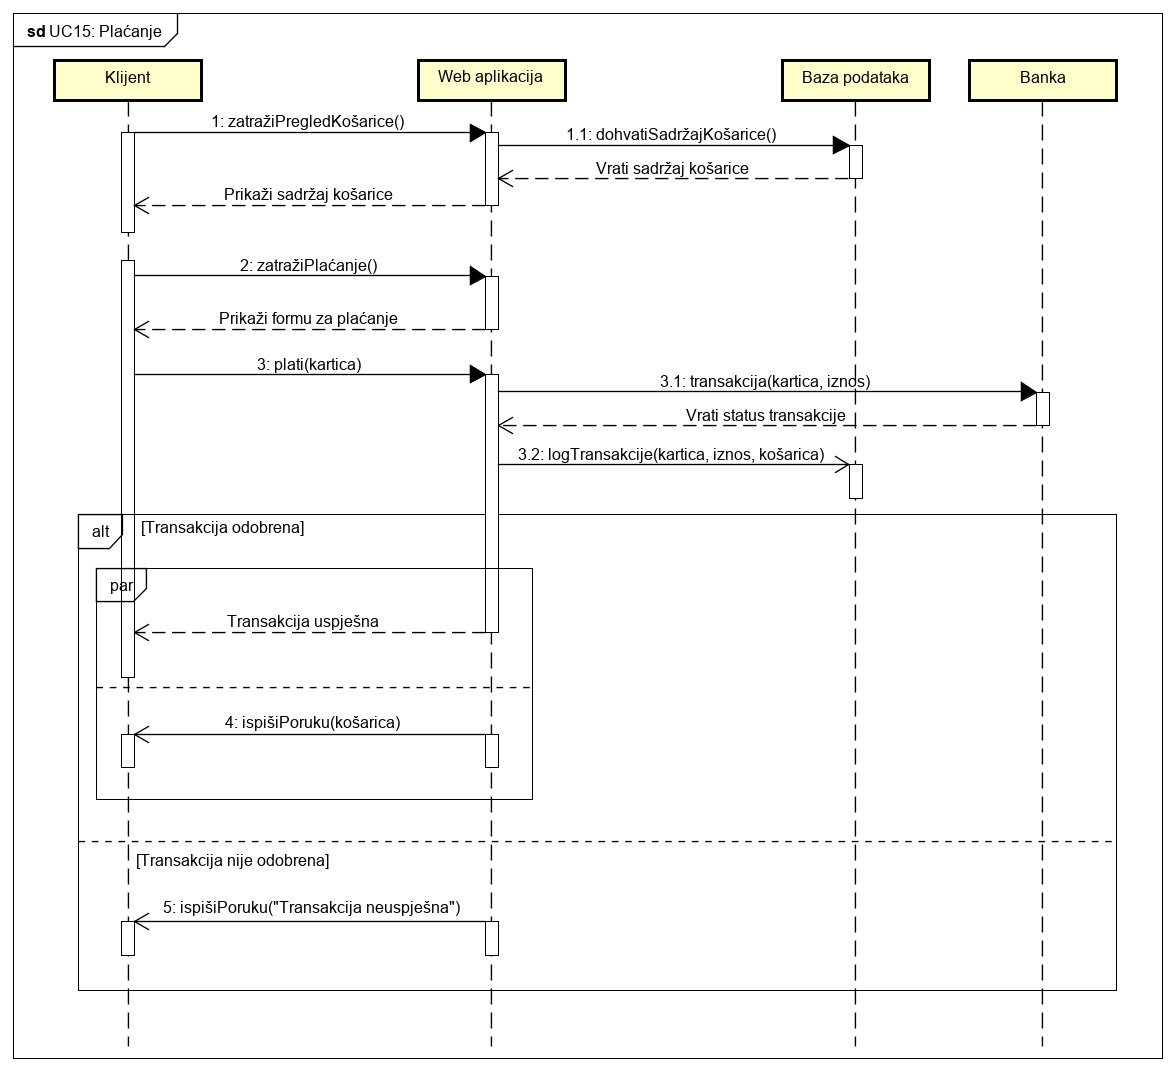
\includegraphics[width=\linewidth]{dijagrami/UC15.png}
					\centering
					\caption{UC15, Plaćanje}
					\label{fig:SequanceDiagram2}
				\end{figure}
			
				\begin{figure}[H]
					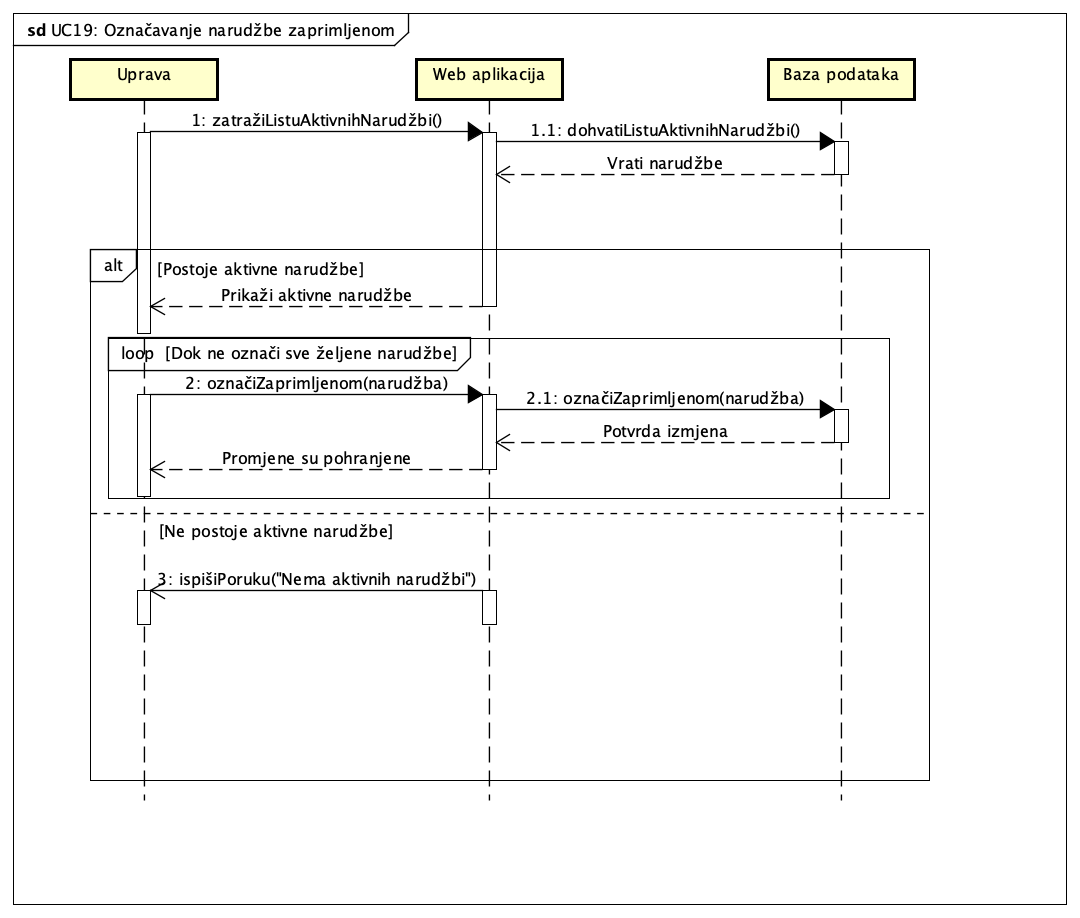
\includegraphics[width=\linewidth]{dijagrami/UC19.png}
					\centering
					\caption{UC19, Označavanje narudžbe gotovom}
					\label{fig:SequanceDiagram3}
				\end{figure}
			
				\begin{figure}[H]
					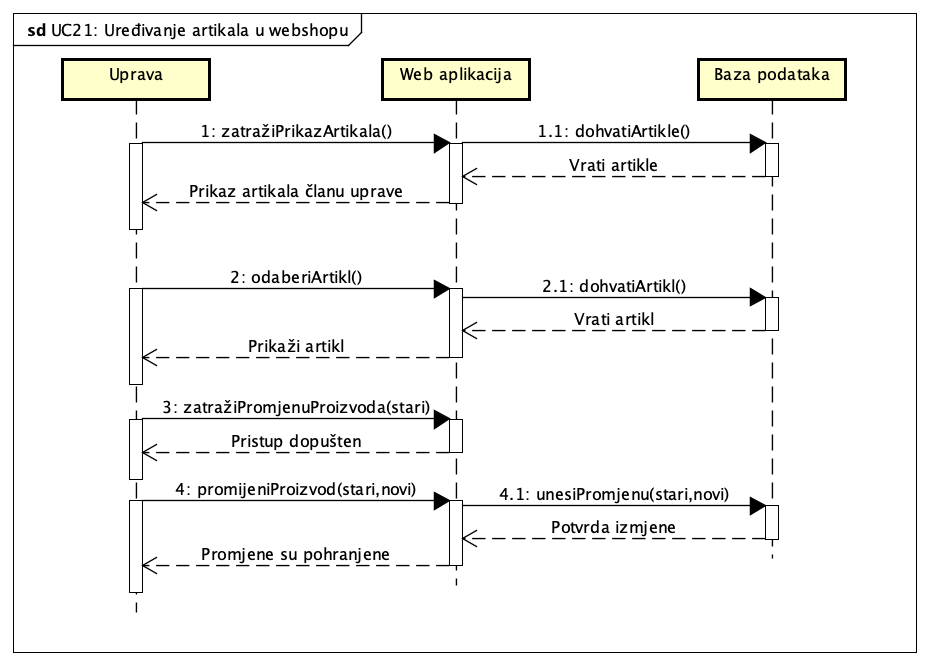
\includegraphics[width=\linewidth]{dijagrami/UC21.png}
					\centering
					\caption{UC21, Uređivanje artikala u web shopu}
					\label{fig:SequanceDiagram4}
				\end{figure}
	
		\section{Ostali zahtjevi}
		
			\begin{packed_item}
				\item Sustav treba omogućiti rad više korisnika u stvarnom vremenu
				\item Korisničko sučelje i sustav moraju podržavati hrvatsku abecedu (dijakritičke znakove) pri unosu i prikazu tekstualnog sadržaja
				\item Izvršavanje dijela programa u kojem se pristupa bazi podataka ne smije trajati duže od nekoliko sekundi
				\item Sustav treba biti implementiran kao web aplikacija koristeći objektno-orijentirane jezike
				\item Neispravno korištenje korisničkog sučelja ne smije narušiti funkcionalnost i rad sustava
				\item Sustav treba biti jednostavan za korištenje, korisnici se moraju znati koristiti sučeljem bez opširnih uputa
				\item Nadogradnja sustava ne smije narušavati postojeće funkcionalnosti sustava
				\item Sustav kao valutu koristi HRK
				\item Veza s bazom podataka mora biti kvalitetno zaštićena, brza i otporna na vanjske greške
				\item Front-end web aplikacije bit će implementiran uz pomoć HTML5, CSS3, Bootstrap 4 i Vue.js tehnologija
				\item Back-end web aplikacije bit će implementiran u programskom jeziku C\#
				\item Čitav sustav će biti utemeljen na okviru rada ASP.NET Core 3.0
				\item Sustav će podržavati hrvatski i engleski jezik
			\end{packed_item}

			 
			 
			 
	